\documentclass[xcolor=dvipsnames]{beamer}
\usepackage{lmodern}
\usepackage[T1]{fontenc}
\usepackage[english]{babel}
\usepackage[utf8]{inputenc}

\usepackage{manfnt}
\usepackage{wasysym}
\usepackage{listings}
\usepackage{graphicx}
\usepackage{url}
\usepackage{ulem}
\usepackage{wasysym}
\usepackage{marvosym}
\usepackage{skull}
\usepackage{proof}
\usepackage{array}
\usepackage{colortbl}
\setbeamertemplate{navigation symbols}{}

\title[Landslide]{{\bf Stateless Model Checking \\ with Data-Race Preemption Points}}
%\subtitle[]{CALCM group seminar}
\author[Ben Blum]{Ben Blum \texttt{(bblum@andrew.cmu.edu)}}

\institute[]{Carnegie Mellon University - CALCM group seminar}
\date[]{2016, March 01}

\setbeamertemplate{footline}{\hspace*{.5cm}\scriptsize{\insertauthor\hspace*{50pt} \hfill\insertframenumber\hspace*{.5cm}}} 

\usecolortheme{seahorse}
\usecolortheme{rose}
\useoutertheme{infolines}

\usecolortheme[named=ForestGreen]{structure}

\newcommand\noob{\mathsf{noob}}
\newcommand\gibs{\mathsf{gibs}}
\newcommand\dps{\mathsf{dps}}
\newcommand\squig\rightsquigarrow
\newcommand\Coloneqq{\mathrel{\mathop{::}}=}
\newcommand\dmg{\text{\Laserbeam}}
\newcommand\delter\delta
\newcommand\alpher\alpha
\newcommand\defnor{\text{ }|\text{ }}

\newcommand\pimp{\mathop{\supset}}
\newcommand\pand{\mathop{\wedge}}
\newcommand\por{\mathop{\vee}}
\newcommand\ptrue{\top}
\newcommand\pfalse{\bot}

\newcommand\hilight[2]{\color{#1}#2\color{black}}
\definecolor{olivegreen}{RGB}{0,127,0}

\begin{document}
\renewcommand{\inserttotalframenumber}{32}
\normalem
\begin{frame}
	\titlepage
\end{frame}

%%%%%%%%%%%%%%%%%%%%%%%%%%%%%%%%%%%%%%%%%%%%%%%%%%%%%%%%%%%%%%%%%%%%%%%%%%%%%%%%
%%%%%%%%%%%%%%%%%%%%%%%%%%%%%%%%%%%%%%%%%%%%%%%%%%%%%%%%%%%%%%%%%%%%%%%%%%%%%%%%
%%%%%%%%%%%%%%%%%%%%%%%%%%%%%%%%%%%%%%%%%%%%%%%%%%%%%%%%%%%%%%%%%%%%%%%%%%%%%%%%

\newcommand\linegap{\vspace{0.2in}}
\newcommand\breakslide[1]{\begin{frame}{} \begin{center} #1 \end{center} \end{frame}}

\begin{frame}{}
	Working on OOPSLA submission (March 23)
	\linegap

	Feedback wanted on:
	\begin{itemize}
		\item What do OOPSLA reviewers look for?
		\item Collaboration and/or ideas for future work
	\end{itemize}
\end{frame}

\begin{frame}{Outline}
	\textbf{Background}
	\begin{itemize}
		\item Preemption points
		\item Stateless model checking (aka, systematic testing)
		\item Data races
	\end{itemize}
	{\bf Quicksand \& Iterative Deepening}
	\begin{itemize}
		\item State space estimation
		\item Data-race preemption points
		\item Implementation with Landslide
	\end{itemize}
	{\bf Evaluation}
	\begin{itemize}
		\item Comparison to ``single-state-space'' approach
		\item Nondeterministic data-race candidates
		\item Providing total verification
	\end{itemize}
\end{frame}


\section{Introduction}

\subsection{Stateless Model Checking}
\definecolor{thread1}{RGB}{87,172,255}
\definecolor{thread2}{RGB}{255,201,102}
\definecolor{thread3}{RGB}{255,128,160}

\begin{frame}{Case Study}
	\begin{center}
		\begin{tabular}{llll}
			\fbox{
			\begin{tabular}{l}
				Consumer thread \\
				\hline
				\\
				\texttt{mutex\_lock(mx);} \\
				\\
				\texttt{if~(!work\_exists())} \\
				\texttt{~~~~cond\_wait(cvar,~mx);} \\
				\texttt{work~=~dequeue();} \\
				\\
				\texttt{mutex\_unlock(mx);} \\
				\texttt{access(work->data);} \\
			\end{tabular}
			}
			& & &
			\fbox{
			\begin{tabular}{l}
				Producer thread \\
				\hline
				\\
				\texttt{mutex\_lock(mx);} \\
				\\
				\texttt{enqueue(work);} \\
				\texttt{signal(cvar);} \\
				\\
				\texttt{mutex\_unlock(mx);} \\
				\\
				\\
			\end{tabular}
			}
		\end{tabular}
		\linegap

		\begin{itemize}
			%\item See {\bf Paradise Lost} lecture!
			\item {\tt if} vs {\tt while}: Two consumers can interleave to make one fail.
		\end{itemize}
	\end{center}
\end{frame}
\begin{frame}{Thread Interleavings (``good'' case)}
	\begin{center}
		\begin{tabular}{|l|l|l|}
			\hline
			\cellcolor{thread1} {\bf Thread 1} & \cellcolor{thread2} {\bf Thread 2} & \cellcolor{thread3} {\bf Thread 3} \\
			\hline
			\small \texttt{lock(mx);} & & \\
			\small \texttt{if~(!work\_exists())} & & \\
			\small \texttt{~~~~wait(cvar,~mx);} & & \\
			
			& & \small \texttt{lock(mx);} \\
			& & \small \texttt{if~(!work\_exists())} \\
			& & \small \texttt{~~~~wait(cvar,~mx);} \\

			& \small \texttt{lock(mx);} & \\
			& \small \texttt{enqueue(work);} & \\
			& \small \texttt{signal(cvar);} & \\
			& \small \texttt{unlock(mx);} & \\
			
			\small \texttt{work~=~dequeue();~} & & \\
			\small \texttt{unlock(mx);} & & \\
			\small \texttt{access(work->data);}& & \\
			\hline
		\end{tabular}
	\end{center}
\end{frame}
\begin{frame}{Thread Interleavings (different ``good'' case)}
	\begin{center}
		\begin{tabular}{|l|l|l|}
			\hline
			\cellcolor{thread1} {\bf Thread 1} & \cellcolor{thread2} {\bf Thread 2} & \cellcolor{thread3} {\bf Thread 3} \\
			\hline
			\small \texttt{lock(mx);} & & \\
			\small \texttt{if~(!work\_exists())} & & \\
			\small \texttt{~~~~wait(cvar,~mx);} & & \\
			
			& \small \texttt{lock(mx);} & \\
			& \small \texttt{enqueue(work);} & \\
			& \small \texttt{signal(cvar);} & \\
			& \small \texttt{unlock(mx);} & \\
			
			\small \texttt{work~=~dequeue();~} & & \\
			\small \texttt{unlock(mx);} & & \\
			\small \texttt{access(work->data);}& & \\
			
			& & \small \texttt{lock(mx);} \\
			& & \small \texttt{if~(!work\_exists())} \\
			& & \small \texttt{~~~~wait(cvar,~mx);} \\
			\hline
		\end{tabular}
	\end{center}
\end{frame}
\begin{frame}{Thread Interleavings (race condition)}
	\begin{center}
		\begin{tabular}{|l|l|l|}
			\hline
			\cellcolor{thread1} {\bf Thread 1} & \cellcolor{thread2} {\bf Thread 2} & \cellcolor{thread3} {\bf Thread 3} \\
			\hline
			\small \texttt{lock(mx);} & & \\
			\small \texttt{if~(!work\_exists())} & & \\
			\small \texttt{~~~~wait(cvar,~mx);} & & \\
			
			& \small \texttt{lock(mx);} & \\
			& \small \texttt{enqueue(work);} & \\
			& \small \texttt{signal(cvar);} & \\
			& \small \texttt{unlock(mx);} & \\
			
			& & \small \texttt{lock(mx);} \\
			& & \small \texttt{work~=~dequeue();~~} \\
			& & \small \texttt{unlock(mx);} \\

			\small \texttt{work~=~dequeue();} & & \\
			\small \texttt{unlock(mx);} & & \\
			\small \texttt{//~SIGSEGV} {\large \frownie}& & \\
			\hline
		\end{tabular}
	\end{center}
\end{frame}

\newcommand\related[1]{\textsuperscript{\em [#1]}}


\begin{frame}{Motivating Stateless Model Checking}
	Goal: Test as many interleavings as you can (given some CPU budget)
	\linegap

	\textbf{Stress testing}
	\begin{itemize}
		\item Relies on randomly-occurring timer (or I/O) interrupts
			% to perturb threads
		\item Exposes nondeterministic bugs at random
		\item Might not find bugs in any bounded time
	\end{itemize}
	\linegap

	\textbf{Stateless Model Checking} (MC)\related{Godefroid '97}
	\begin{itemize}
		\item Exhaustively exercise {\em all} thread interleavings
		\begin{itemize}
			\item ...around a given set of {\em preemption points}
		\end{itemize}
		\item Identify bugs for certain (e.g. segfault, deadlock, panic)
		\item More reliable coverage, better reproducibility
		\item Exponentially-sized state space of interleavings
			%depending on \# of preemption points
	\end{itemize}
	%Moving beyond stress testing: which {\em preemption points} are important?
\end{frame}

\begin{frame}{Preemption Points}
	\textbf{Preemption points} (PPs) are program locations where a context switch might expose different behaviour.
	\linegap

	Stateless MC is {\em parameterized} by which PPs can trigger thread switches.
	\linegap

	For case study, {\tt mutex\_lock}, {\tt mutex\_unlock}, {\tt cond\_wait} are relevant.
	\pause
	\linegap

	Which PPs to use?
	\begin{itemize}
		\item Every instruction (exhaustive, but intractable)
		\item Synchronization API calls\related{Musuvathi '08, Simsa '10, Blum '12}
		%\item Kernel mutex interface\related{Blum '12}
		\item Global/heap memory accesses\related{Holzmann '97, Yang '08}
	\end{itemize}
\end{frame}

\begin{frame}{MC State of the Art}{(my new DJ name?)}
	Modern stateless MC tools can {\em mitigate} exponential explosion.
	\begin{itemize}
		\item Dynamic Partial Order Reduction (DPOR)\related{Flanagan '05}
		\item State space estimation\related{Simsa '12}
	\end{itemize}
	\linegap

	However, existing MCs ``hard-code'' their PPs in advance.
	\begin{itemize}
		\item With too many preemption points, tests time out.
		\item Which PPs are ``good'' differs for each test case.
		\item Relationship between PPs and testing time is unpredictable.
	\end{itemize}
	\linegap

	Current MC model is not user-friendly.
	\begin{itemize}
		\item Tool: ``I want to use these PPs, but can't predict completion time.''
		\item User: ``I have 16 CPUs and 24 hours to test my program.''
	\end{itemize}
\end{frame}

%%%%%%%%%%%%%%%%%%%%%%%%%%%%%%%%%%%%%%%%%%%%%%%%%%%%%%%%%%%%%%%%%%%%%%%%%%%%%%%%

\subsection{Data Races}

\begin{frame}{Data Races\related{Savage '97}}
	A {\bf data race} is a pair of memory accesses between two threads, where:
	\begin{itemize}
		\item At least one of the accesses is a write
		\item The threads are not holding the same mutex
		%\item The threads can be reordered (e.g., no \texttt{cond\_signal()} in between)
		\item The threads' executions are not related by {\em Happens-Before}
	\end{itemize}

	Data races are {\em not necessarily} bugs, just highly suspicious!
	\begin{itemize}
		\item ``If threads interleaved the wrong way here, it {\em might} crash later.''
		\item Hence, data race locations are ideal PP candidates.
	\end{itemize}
\end{frame}

\begin{frame}{The Happens-Before (HB) Relation}
	Most data-race analyses use {\em Pure HB} to determine simultaneity.
	\begin{itemize}
		\item HB is established by any synchronization (mutexes, cvars, xchg...)
		\item Represents possiblity of threads' behaviour to change if reordered
			%\begin{itemize}
			%	\item ...that the programmers obviously intended.
			%\end{itemize}
		\item May exclude some races from alternate interleavings ({\em false negatives})
	\end{itemize}
	\pause
	\linegap

	To avoid false negatives, we use {\em Limited HB}\related{O'Callahan '03} instead.
	%, Serebryany '09}
	\begin{itemize}
		\item HB is established only when thread runnability changes (cvars).
		\item Represents ability to reorder accesses to occur simultaneously
		\item Captures accesses separated by unrelated, synchronized, logic
		\item Will also falsely flag some {\em false positives}
		\item Combined with lock-set analysis to increase accuracy
	\end{itemize}
\end{frame}


\begin{frame}{Happens-Before Example}
	\begin{center}
		\begin{tabular}{|l|l|}
			\hline
			\cellcolor{thread1} {\bf Thread 1} & \cellcolor{thread2} {\bf Thread 2} \\
			\hline
			& \\
			\small \texttt{x++;} // A & \\
			\small \texttt{lock(mx);} & \\
			%\small \texttt{y = true;} & \\
			\small \texttt{unlock(mx);} & \\
			
			& \\
			& \small \texttt{lock(mx);} \\
			& \small \texttt{unlock(mx);} \\
			& \small \texttt{x++;} // B \\
			& \\
			\hline
		\end{tabular}
	\end{center}
	{\bf Pure HB}: \texttt{mx} establishes $HB(A, B)$; no race reported (false negative).
	\linegap

	{\bf Limited HB}: $\neg HB(A, B)$; race is reported (correctly).
\end{frame}

\begin{frame}{Happens-Before Example}
	\begin{center}
		\begin{tabular}{|l|l|}
			\hline
			\cellcolor{thread1} {\bf Thread 1} & \cellcolor{thread2} {\bf Thread 2} \\
			\hline
			\small \texttt{x++;} // A & \\
			\small \texttt{lock(mx);} & \\
			\small \texttt{y = true;} & \\
			\small \texttt{unlock(mx);} & \\
			
			& \small \texttt{lock(mx);} \\
			& \small \texttt{bool z = y;} \\
			& \small \texttt{unlock(mx);} \\
			& \small \texttt{if (z);} \\
			& \small \texttt{~~x++;} // B \\
			\hline
		\end{tabular}
	\end{center}
	{\bf Pure HB}: \texttt{mx} establishes $HB(A, B)$; no race reported (correctly).
	\linegap

	{\bf Limited HB}: $\neg HB(A, B)$; race is reported (false positive).
\end{frame}

%%%%%%%%%%%%%%%%%%%%%%%%%%%%%%%%%%%%%%%%%%%%%%%%%%%%%%%%%%%%%%%%%%%%%%%%%%%%%%%%

\breakslide{\Huge Quicksand}

\begin{frame}{Iterative Deepening of Preemption Points}
	Goal: Run the best tests for a given CPU budget.
	\linegap

	Inspired by past experience with Landslide, our MC tool\related{Blum '12}
	\begin{itemize}
		\item 15-410 student volunteers worked best with iterative process
		\item ``Start small, then add more preemption points as time allows''
		\item Quicksand now automates this via {\em Iterative Deepening}
	\end{itemize}
	\linegap

	Named after analogous technique in chess AI.
	\begin{itemize}
		\item Chess search is DFS limited by max number of moves (ply).
		\item Chess AIs repeat DFS, increasing ply, until timeout.
	\end{itemize}
\end{frame}

\begin{frame}{Iterative Deepening in Quicksand}
	Quicksand automatically iterates through different configurations of PPs.
	\begin{itemize}
		\item Manages work queue of jobs with different PPs
		\item Each job represents a new state space for Landslide to explore
		\item Prioritizes jobs based on estimated completion time
		%\item Prioritizes which jobs are important / likely to finish
		%\begin{itemize}
		%	\item Based on nature of PPs (data races? mutexes?)
		%	\item Based on estimated completion time
		%\end{itemize}
		\item New PPs added on-the-fly from data-race analysis
	\end{itemize}
	\linegap

	Repeat state space explorations, adding preemption points, until time is exhausted.

	\linegap
	{\em Only required argument is CPU budget}
\end{frame}

\begin{frame}{Iterative Deepening}
	Minimal state space includes only ``mandatory'' context switches
	\begin{itemize}
		\item e.g., {\tt yield()}, {\tt cond\_wait()}.
		% Say: When the test invokes yield, the kernel scheduler will pick
		% one thread to run next. With Landslide, we will pick ALL threads to
		% run next, in one parallel universe at a time.
	\end{itemize}
	\vspace{0.29in}
	\begin{center}
		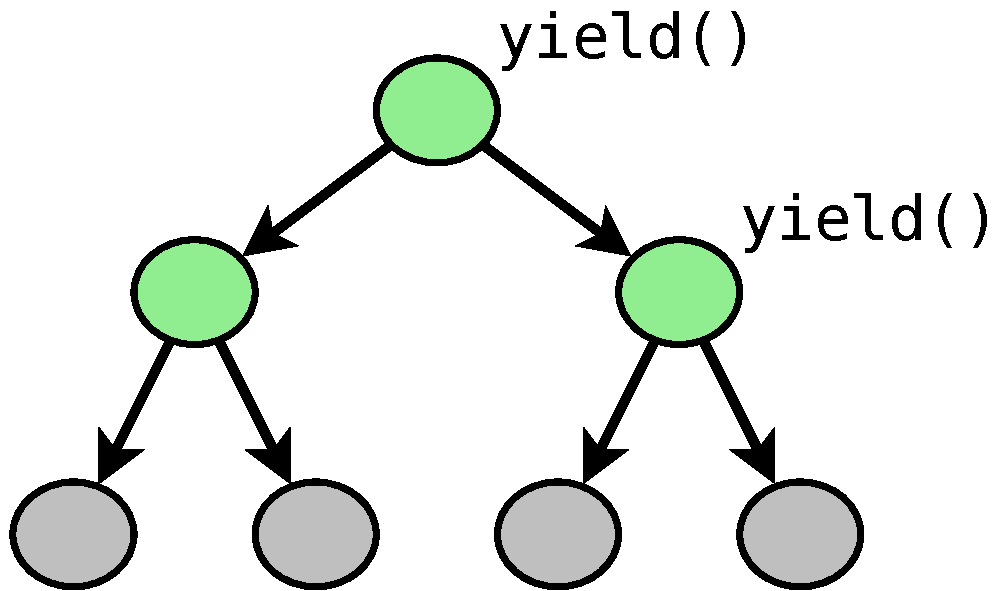
\includegraphics[width=0.35\textwidth]{tree0.pdf}
	\end{center}
\end{frame}

\begin{frame}{Iterative Deepening}
	Adding different PPs can produce state spaces of different sizes; Quicksand tries them in parallel, as informed by state space estimation\related{Simsa '12}.
	\vspace{0.15in}
	\begin{center}
		\begin{tabular}{cc}
			\includegraphics[width=0.45\textwidth]{tree1.pdf} &
			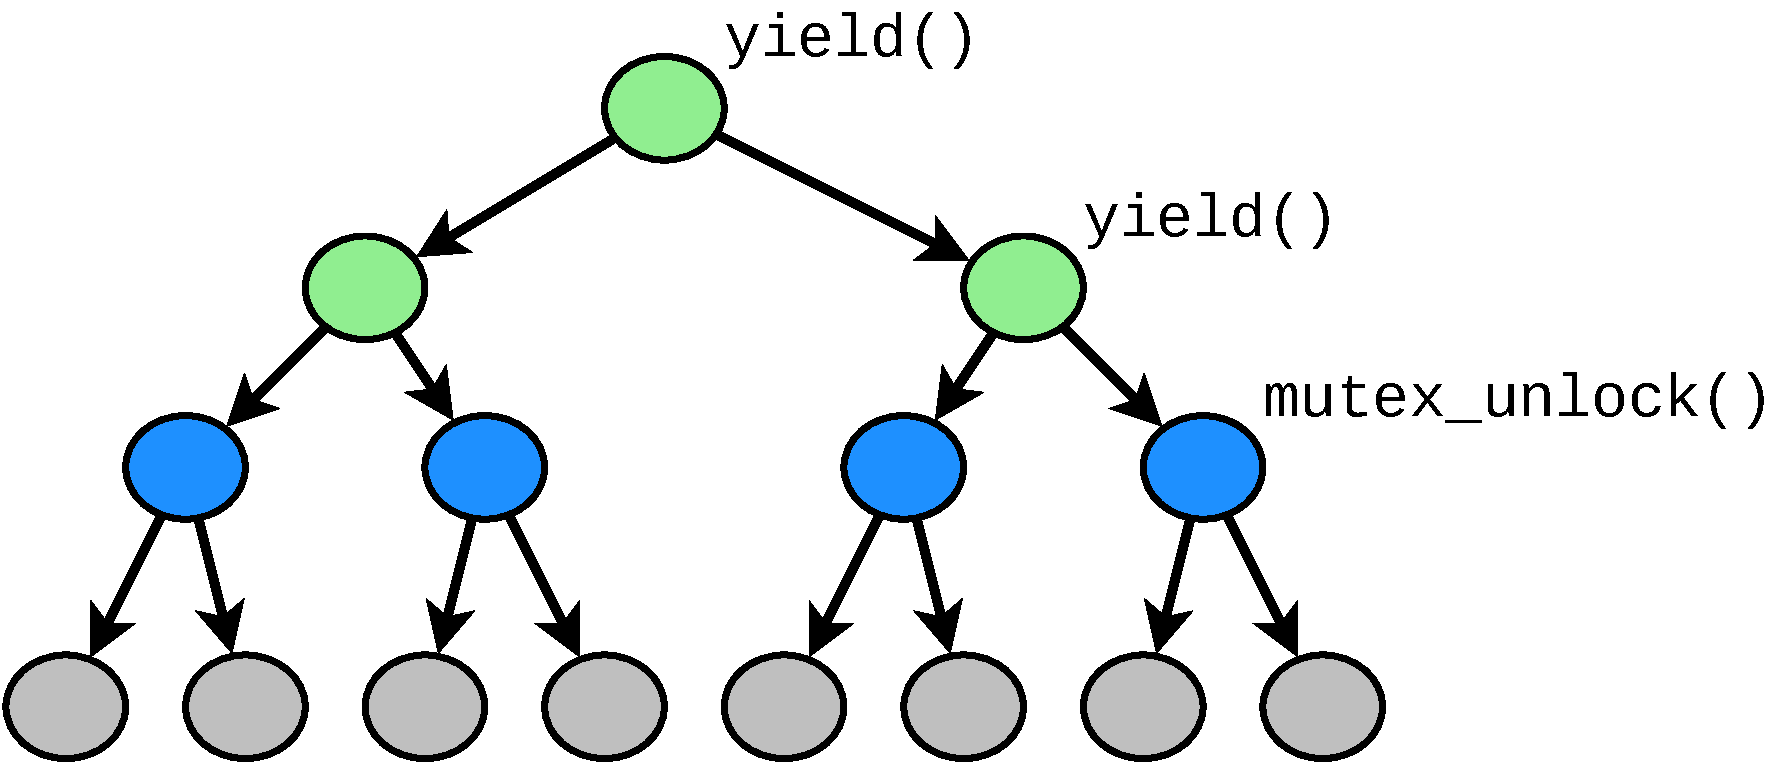
\includegraphics[width=0.5\textwidth]{tree2.pdf}
		\end{tabular}
	\end{center}
\end{frame}


\begin{frame}{Iterative Deepening}
	If time allows, combine PPs into larger, more comprehensive state spaces.
	\linegap

	All PPs enabled = ``maximal'' state space
	\begin{itemize}
		\item Prior work tools test this state space only.
	\end{itemize}
	%eventually converging to using all PPs at once ({\em ``maximal'' state space}).
	\begin{center}
		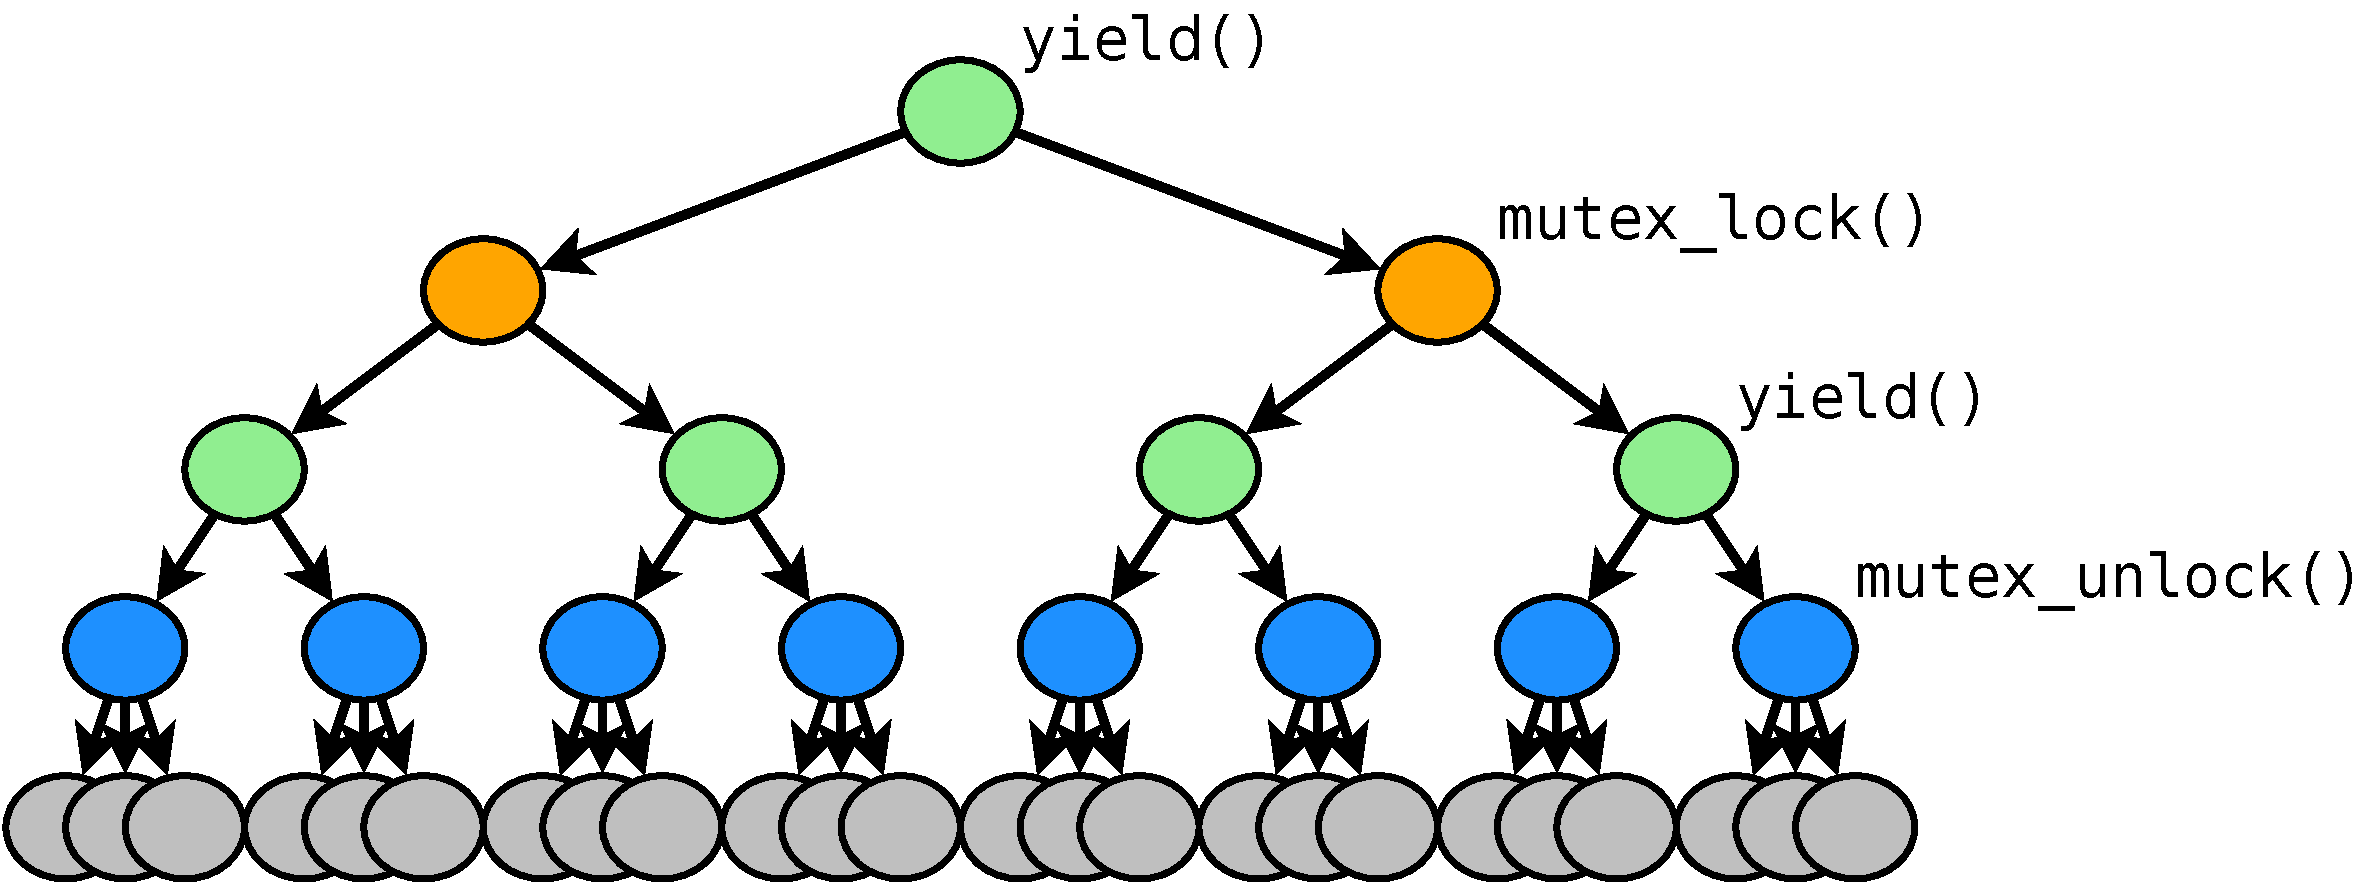
\includegraphics[width=0.8\textwidth]{tree3.pdf}
	\end{center}
	% say: and depending on your time budget, you might decide that you expect this one to be feasible, or you might fall back to a smaller state space from before.
\end{frame}

\begin{frame}{Total Verification}
	% Let's come back to this issue of ...
	MC can {\em totally verify} a test by testing a state space with all possible PPs.
	\begin{itemize}
		\item Ordinarily infeasible, but some tests are small enough
		%\item Whether a test can be totally verified can't be known in advance.
		\item ``Hard-coded'' PP approach\related{Musuvathi '08} sacrifices this possibility.
	%One downside of hard-coding PPs in advance is timing out when the test is too large, but another downside is if the test is small enough, you might miss a possible full verification!
		\item What PP strategy works for both small and large tests?
	\end{itemize}
	\pause
	\linegap

	Synchronization API PPs \& data-race PPs are sufficient!
	\begin{itemize}
		\item {\bf Theorem (Convergence)}:
			{\em If a bug can be exposed by any thread interleaving
				possible by preempting on all instructions,
				% during a specific test
			Quicksand will eventually test an equivalent interleaving which exposes the same bug.}
		\item Proof appeals to DPOR soundness\related{Flanagan '05} and Limited HB.
		\item Intuition: ``Adding data-race PPs until saturation = all possible thread communication points.''
	\end{itemize}
\end{frame}


%%%%%%%%%%%%%%%%%%%%%%%%%%%%%%%%%%%%%%%%%%%%%%%%%%%%%%%%%%%%%%%%%%%%%%%%%%%%%%%%
%%%%%%%%%%%%%%%%%%%%%%%%%%%%%%%%%%%%%%%%%%%%%%%%%%%%%%%%%%%%%%%%%%%%%%%%%%%%%%%%
%%%%%%%%%%%%%%%%%%%%%%%%%%%%%%%%%%%%%%%%%%%%%%%%%%%%%%%%%%%%%%%%%%%%%%%%%%%%%%%%
%%%%%%%%%%%%%%%%%%%%%%%%%%%%%%%%%%%%%%%%%%%%%%%%%%%%%%%%%%%%%%%%%%%%%%%%%%%%%%%%

\section{Evaluation}

\breakslide{\Huge Evaluation}

\begin{frame}{Evaluation}
	Evaluation questions:
	\begin{enumerate}
		\item Do we find more bugs than prior MC with data-race PPs?
		\item Do we find bugs faster than prior MC, even without data-race PPs?
			% say: "the same bugs"
		\item Does MC uncover new, nondeterministic, data-race candidates?
		\item Do we provide more total verifications than prior MC?
	\end{enumerate}
\end{frame}

\begin{frame}{Experimental Setup}
	\textbf{Test suite}: 79 ``P2''s $\times$ 6 test cases + 78 ``Pintos''s $\times$ 3 test cases
	\begin{itemize}
		\item P2: CMU 15-410 thread library project (\textasciitilde{}1800 LOC)
		\item Pintos: Berkeley CS162/U. Chicago CS320 kernel project (\textasciitilde{}700 LOC)
		\item 629 unique state spaces (i.e., project/test pairs)
	\end{itemize}
\end{frame}
\begin{frame}{Experimental Setup}
	\textbf{Quicksand experiment}: 1 hour $\times$ 10 CPUs per test
	\begin{itemize}
		\item {\bf QS}: Data-race PPs enabled
		\item {\bf QS-no-DRs}: Restrict iterative deepening to sync API PPs only
	\end{itemize}
	\linegap

	{\bf Control experiment}: 10 hours $\times$ 1 CPU per test
	\begin{itemize}
		\item Test only ``maximal`` state space, using all sync API PPs at once
		\item {\bf DPOR}: Use DPOR\related{Flanagan '05} to test maximal space in single pass
		\item {\bf ICB}: Use Iterative Context Bounding\related{Musuvathi '07, Coons '13} to repeatedly test maximal space with increasing preemption bound
			% dont mention BPOR
	\end{itemize}
\end{frame}

\begin{frame}{1. Finding more bugs with data-race PPs}
	\begin{center}
		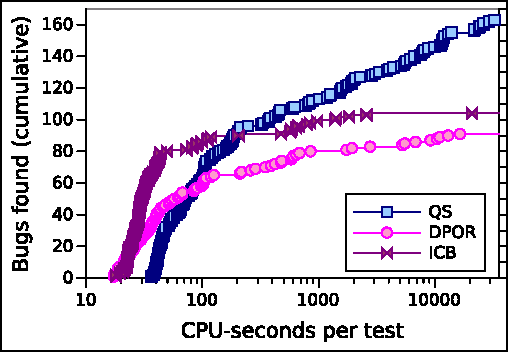
\includegraphics[width=0.6\textwidth]{eval1.pdf}
	\end{center}
	\begin{itemize}
		\item 17-118 seconds: Quicksand loses on parallelization/startup overhead
			%\begin{itemize}
			%	\item (remember: Quicksand on 10 CPUs, control on 1)
			%\end{itemize}
		\item Ultimately, 180\% as many bugs in total!
	\end{itemize}
\end{frame}

\begin{frame}{2. Finding the same bugs... slower}
	\begin{center}
		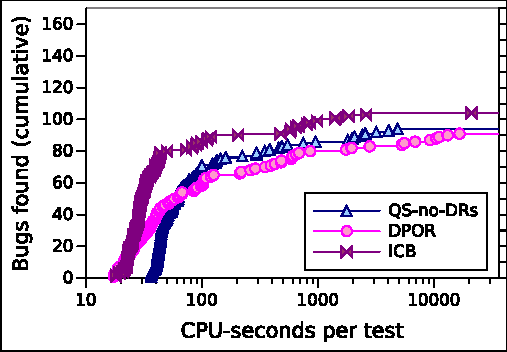
\includegraphics[width=0.6\textwidth]{eval2.pdf}
	\end{center}
	\begin{itemize}
		\item ICB outperforms Iterative Deepening when using the same PPs
		\item Suggests Quicksand could incorporate ICB in its scheduling strategy
	\end{itemize}
\end{frame}

\begin{frame}{3. Nondeterministic data-race candidates}
	Some data races come from code that executes only nondeterministically.
	\begin{itemize}
		\item In a single-execution data race analysis, these accesses won't be seen.
		\item MC can uncover the racy logic, identify a new PP, and find more bugs.
	\end{itemize}

	\begin{center}
		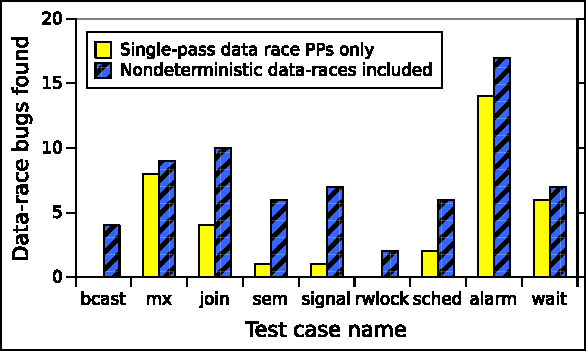
\includegraphics[width=0.7\textwidth]{eval3.pdf}
	\end{center}
\end{frame}

\begin{frame}{4. Total verification}
	\begin{center}
		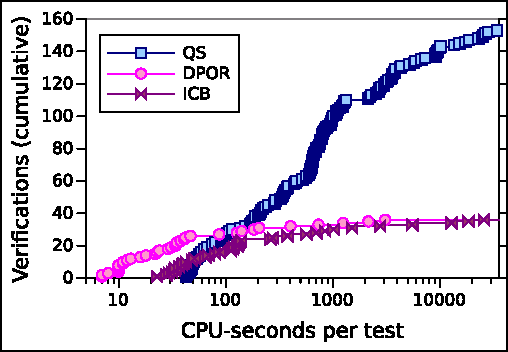
\includegraphics[width=0.6\textwidth]{eval4.pdf}
	\end{center}
	\begin{itemize}
		\item If no data-race candidates, can verify with sync API PPs alone.
		\item Data-race PPs allow total verification of 425\% as many tests!
		\item ICB slower to verify than single-pass DPOR due to repeated work.
	\end{itemize}
\end{frame}

%%%%%%%%%%%%%%%%%%%%%%%%%%%%%%%%%%%%%%%%%%%%%%%%%%%%%%%%%%%%%%%%%%%%%%%%%%%%%%%%

\section{End}
\breakslide{\Huge Conclusion}

\begin{frame}{Conclusion}
	Stateless Model Checking depends on good {\bf preemption points} (PPs).
	\linegap

	MC State of the Art chooses a fixed PP set in advance.
	\linegap

	Quicksand schedules multiple tests, with different PPs, in parallel.
	\begin{itemize}
		\item Iterative Deepening incorporates new data-race PPs on-the-fly
		\item Data race PPs uncover {\bf 80\% more bugs} than sync API PPs alone
		\item Data race PPs enable {\bf total verification} when test is small enough
	\end{itemize}
	\linegap

	OOPSLA submission soon; looking for feedback!
\end{frame}

\breakslide{\Large Questions?
\linegap

\begin{center}
	\includegraphics[width=0.65\textwidth]{3word-questions.png}
\end{center}}

%%%%%%%%%%%%%%%%%%%%%%%%%%%%%%%%%%%%%%%%%%%%%%%%%%%%%%%%%%%%%%%%%%%%%%%%%%%%%%%%
%%%%%%%%%%%%%%%%%%%%%%%%%%%%%%%%%%%%%%%%%%%%%%%%%%%%%%%%%%%%%%%%%%%%%%%%%%%%%%%%
%%%%%%%%%%%%%%%%%%%%%%%%%%%%%%%%%%%%%%%%%%%%%%%%%%%%%%%%%%%%%%%%%%%%%%%%%%%%%%%%

\section{Bonus Slides}

\end{document}
